\section{Constituitive Models} \label{sec:consituitiveModels}

% ---------------------------------------------------------------------------------
\newcommand{\Cvv}{\underline{\underline{\Cv}}}
\subsection{Elastic strain energy function}

The elastic strain energy function (or {\em elastic strain energy potential}) is denoted by $w$ and is
a measure of the potential energy in a strained elastic material. We will consider
materials for which 
\begin{align*}
   w=w(\Ev).
\end{align*}
The elastic strain energy function is used to define constituitive models for a class of materials.
%
For Kirchoff materials, $w$ is a positive definite quadratic function of $\Ev$, 
\begin{align*}
&   w= \half \Ev \, \Cvv \, \Ev = \half C_{ijkl} E_{ij} E_{kl} , 
              \quad C_{ijkl}=\frac{\partial^2 w}{\partial E_{ij} \partial E_{kl}}
       \qquad\text{(Kirchoff materials)}.\\
&    \Sv = \Cvv\, \Ev , \quad S_{ij} = C_{ijkl} E_{kl}  \qquad\text{(Generalized Hooke's law: Kirchoff materials)}.
\end{align*}
The {\em minor} symmetries of $C_{ijkl}$ (valid for Kirchoff materials) follow from $\Sv = \Cvv\, \Ev$, and 
the symmetry of $\Ev$ and $\Sv$: $C_{ijkl}=C_{jikl}$, ($i\leftrightarrow j$), and $C_{ijkl}=C_{ijlk}$ ($k\leftrightarrow l$).
The {\em major} symmetries (valid for $w=w(\Ev)$) follow from the equality of mixed partials of $w$, $C_{ijkl}=C_{kjil}$ ($i\leftrightarrow k$)
 and $C_{ijkl}=C_{ilkj}$ ($j\leftrightarrow l$). 
%
For Kirchoff and hyperelastic materials (i.e. materials where $w=w(\Ev)$), the PK2 stress, $\Sv$, is related to $w$ by 
\begin{align*}
    \Sv = \frac{\partial w(\Ev)}{\partial\Ev}.
\end{align*}
It follows that the nominal stress $\Pv$ is given by 
\begin{align}
    P_{ij} = \frac{\partial w}{\partial F_{ji}}, \quad \Pv = \frac{\partial w}{\partial\Fv^T}  \label{eq:wToP}
\end{align}
Equation~\eqref{eq:wToP} can be derived using the relations
\begin{align*}
    \frac{\partial w}{\partial F_{ij}} &= \frac{\partial w}{\partial E_{kl}}\, \frac{\partial E_{kl}}{\partial E_{ij}} , \\
     E_{kl} &= \half( F_{\mu k} F_{\mu l} - \delta_{kl} ), \qquad\big( \Ev=\half(\Fv^T \Fv - I)\big) , \\
    \frac{\partial E_{kl}}{\partial E_{ij}} &= \half\Big( \delta_{\mu i}\delta_{j k} \,F_{\mu l} + F_{\mu k}\,\delta_{\mu i}\delta_{l j} \Big) 
              ~= \half\Big( \delta_{j k} F_{i l} + \delta_{l j}F_{i k} \Big) 
\end{align*}
Whence
\begin{align*}
    \frac{\partial w}{\partial F_{ij}} &=\frac{\partial w}{\partial E_{kl}}\, \half\Big( \delta_{j k} F_{i l} + \delta_{l j}F_{i k} \Big) \quad
       = \half\Big( \frac{\partial w}{\partial E_{jl}} F_{i l} + \frac{\partial w}{\partial E_{kj}} F_{i k} \Big) \\
       &= \half\Big( S_{jl}  F_{i l}  + S_{kj} F_{i k} \Big) = \half\Big( S_{jl}  F_{i l}  + S_{jk} F_{i k} \Big)  ~= \half( P_{ji} + P_{ji} )\\
       &= P_{ji}
\end{align*}
where we have used $\Pv=\Sv \Fv^T$ (i.e. $P_{ij}=S_{ik} F_{jk}$). 

Examples:
\begin{alignat*}{3}
&   w = \frac{\lambda}{2} \big[\tr(\Ev)\big]^2 + \mu \tr(\Ev^2)  \qquad && \text{(Saint-Venant Kirchoff)}, \\
&  w(\Ev)= \psi(\Cv) = \half\lambda_0 (\ln(J))^2 - \mu_0 \ln(J) + \half \mu_0(\tr(\Cv)-3), \qquad && \text{(Neo-Hookean)}
\end{alignat*}
where $J=\det(\Fv)$, $\Cv=\Fv^T\Fv=2\Ev+I$ and $w(\Ev)=\psi(2\Ev+I)$.

% ---------------------------------------------------------------------------------
\clearpage
\subsection{Hyperelastic (Green elastic) models}

Hyperelastic materials are those for which the work is independent of the load path (e.g. rubber like material).
They are characterized by by a stored (strain) energy function $\psi(\Cv)$, ($w(\Ev)=\psi(2\Ev+I)$, $\Cv=\Fv^T\Fv$), 
\begin{align*}
    \Sv = 2 \frac{\partial \psi(\Cv)}{\partial \Cv} = \frac{\partial w(\Ev)}{\partial\Ev}
\end{align*}

% ---------------------------------------------------------------------------------
\subsection{Models for large strain and deformation}


In this section we consider how some material models behave for large strains and deformations.

In the article {\em Invertible finite elements for robust simulation of large deformation}
by Irving, Teran and Fediw~\cite{IrvingTeranFedkiw2004}, they note that the SVK model behaves
poorly for large strains and they consider some alternatives.

Recall that in material coordinates $\Xv$ the equations of motion are
\begin{align}
  \rho_0 \partial_t^2 \uv &= \grad_{\Xv}\cdot \Pv, \\
  \rho_0 \partial_t^2 u_i  &= \frac{\partial}{\partial X_j} P_{ji}  
       =  \frac{\partial P_{ji}}{\partial F_{kl}}  \frac{\partial F_{kl}}{\partial X_j} \\
      & = K_{jikl} \frac{\partial^2 u_k}{\partial X_l\partial X_j}, \quad\text{(c.f. Don's $K_{ijkl}$)}, 
\end{align}
where $\Pv=\Pv(\Fv)$ ($\Fv = \Iv + \partial\uv/\partial\xv$) is the nominal stress (first Piola-Kirchoff stress).
Freezing coefficients and substituting $\uv=e^{i\kv\cdot\xv-\omega t}\hat{\uv}$ gives the (matrix) dispersion relation
\begin{align}
   \rho_0 \omega^2 \hat{u}_i  =  K_{jikl} k_l k_j \hat{u}_k,
\end{align}
whose eigenvalues are the wave speeds. 

The SVK model defines $\Pv$ as a function of $\Fv$ by 
\begin{align}
  \Pv &= \Sv \Fv^T,  \\
  \Sv &= \lambda tr(\Ev) I + 2\mu \Ev, \\ 
  \Ev &= \half( \Fv^T \Fv - I).
\end{align}


\newcommand{\Fvhat}{\hat{\Fv}}
\newcommand{\Phat}{\hat{P}}
\newcommand{\Pvhat}{\hat{\Pv}}
The {\em rotated-linear} (RL) model~\cite{IrvingTeranFedkiw2004} can be defined in terms of the singular value decomposition (SVD) of
the deformation gradient tensor $\Fv$, 
\begin{align}
  \Fv &= \Uv \Fvhat \Vv^T \quad{(SVD)} ,  \\
  \Pvhat &= \lambda tr(\Fvhat-\Iv)\Iv + 2\mu( \Fvhat -\Iv), \\ 
  \Pv &= \Uv \Pvhat \Vv^T 
\end{align}


The {\em neo-Hookean} model~\cite{Belytschko2005} is defined in terms of the {\em right Cauchy Green deformation tensor}, $\Cv$, (not
to be confused with the tensor of elastic modulii!)
\begin{align}
   \Cv &= \Fv^T\Fv \quad\text{(right Cauchy Green deformation tensor)},\\
   \Sv &= \lambda \ln(J) \Cv^{-1} + \mu( \Iv - \Cv^{-1} ), \qquad J =\det(\Fv), \\
       &= \lambda \ln(J) \Fv^{-1}\Fv^{-T} + \mu( \Iv - \Fv^{-1}\Fv^{-T} ) , \\
   \Pv &= \Sv \Fv^T =  \lambda \ln(J) \Fv^{-1} + \mu( \Fv^T - \Fv^{-1} ) .
\end{align}
Note that for small $\partial \uv/\partial\Xv$, $\ln(J)\approx tr(\partial \uv/\partial\Xv)$,
and $\Fv^{-1} \approx \Iv - \partial\uv/\partial\Xv$. 


{\newcommand{\graphWidth}{8cm}
\begin{figure}
\begin{center}
  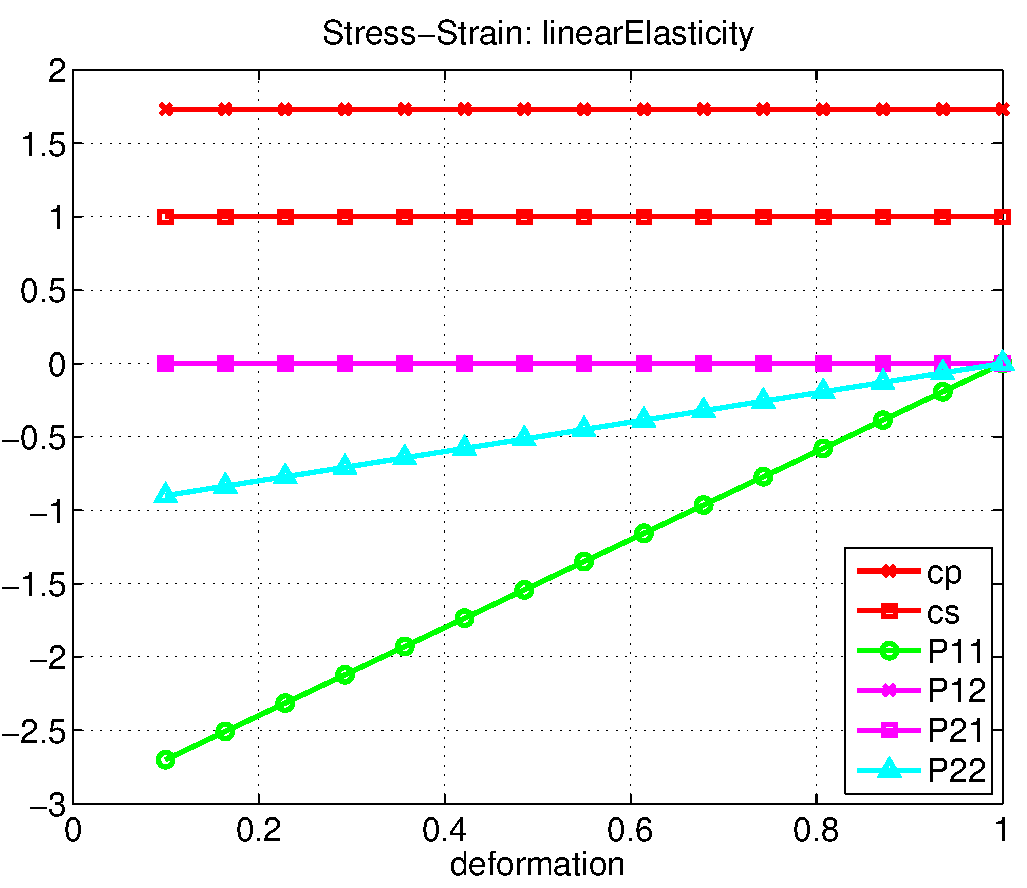
\includegraphics[width=\graphWidth]{fig/linearElasticityStressStrain}
  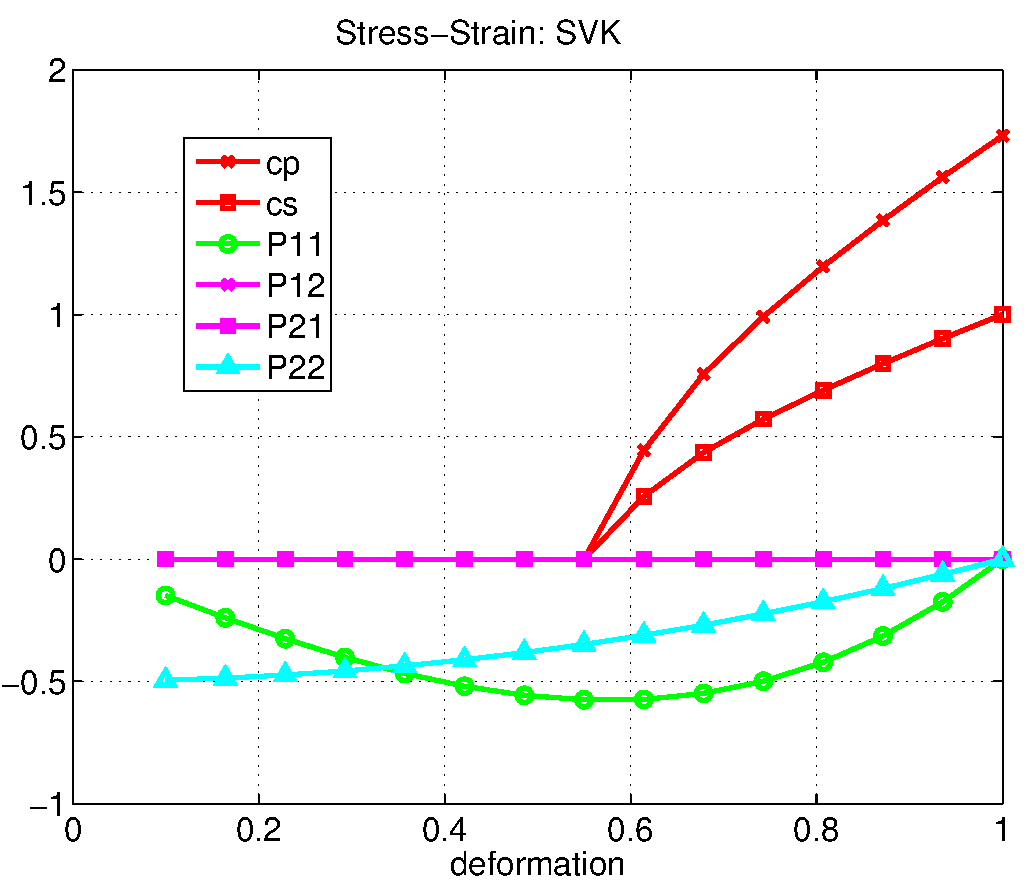
\includegraphics[width=\graphWidth]{fig/SVKStressStrain}
  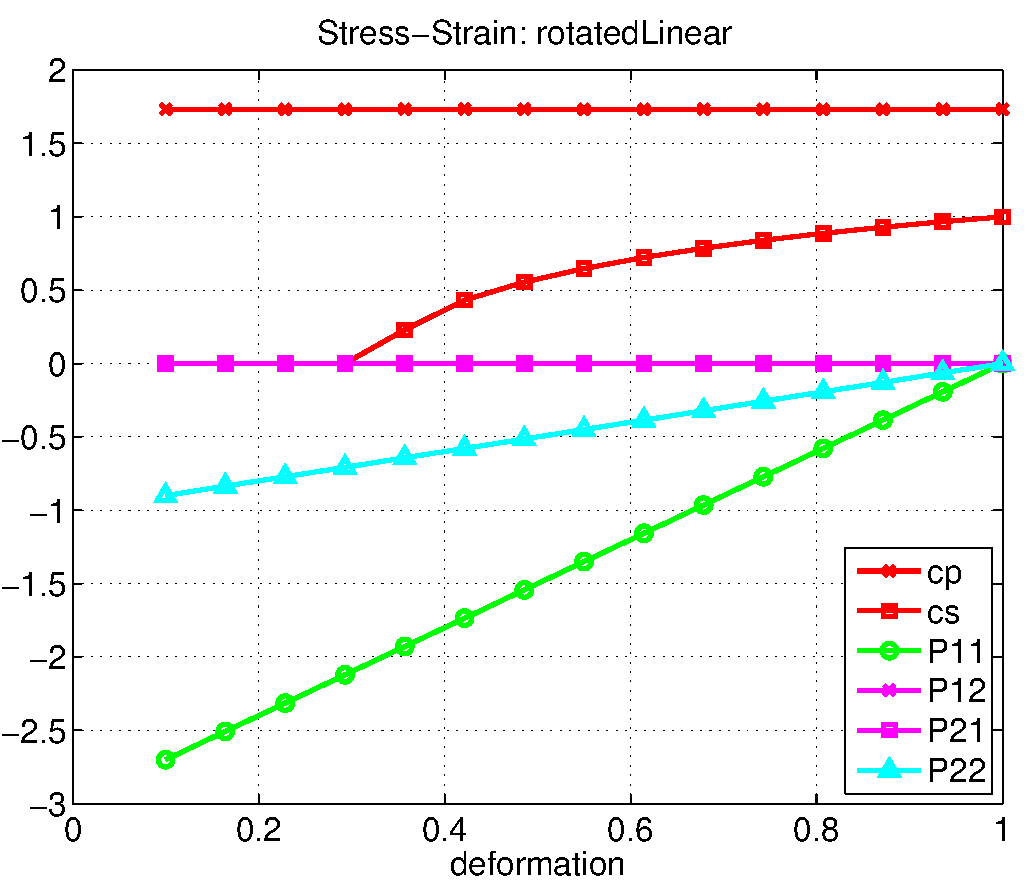
\includegraphics[width=\graphWidth]{fig/rotatedLinearStressStrain}
  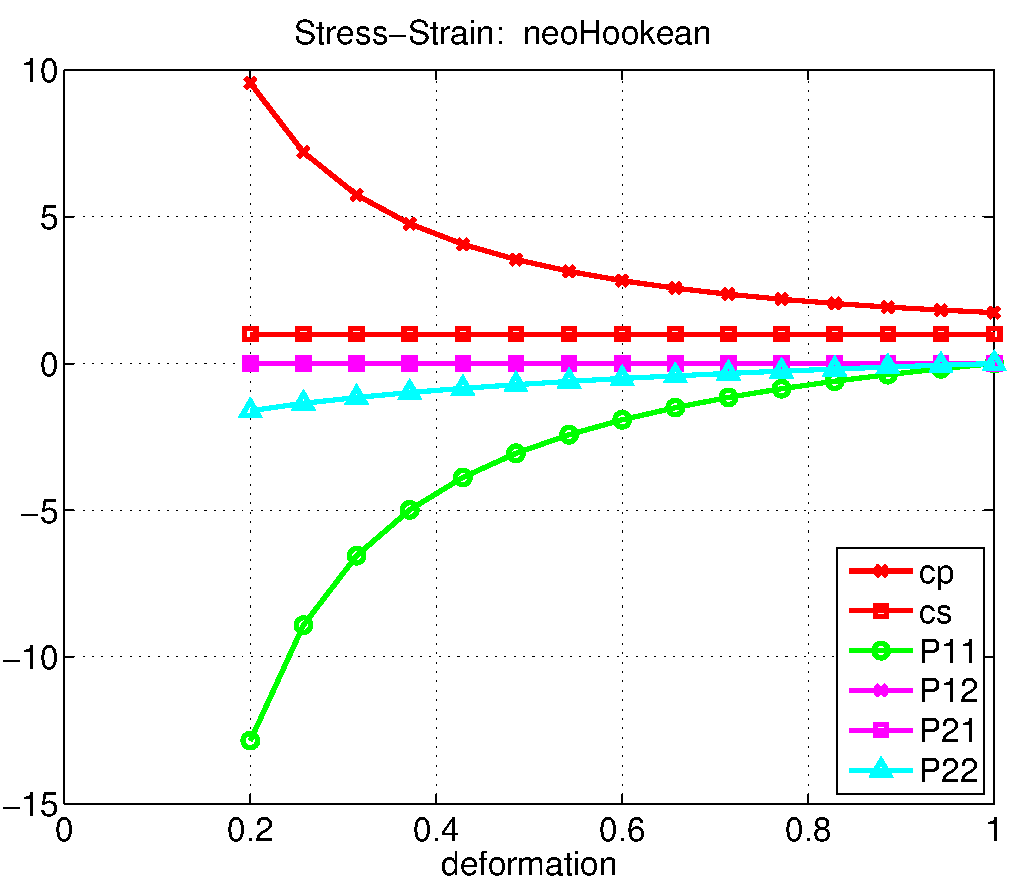
\includegraphics[width=\graphWidth]{fig/neoHookeanStressStrain}
  \caption{Stress strain relationships.}
  \label{fig:largeStressStrain}
\end{center}
\end{figure}
}

The different models are compared in Figure~\ref{fig:largeStressStrain} for $\rho_0=\lambda=\mu=1$. We consider a material under compression
with $\partial u_1/\partial x_1 \le 0$ and all other components of $\partial\uv/\partial\xv$ being zero. 
We plot the components of $\Pv$ as a function of the deformation $f=1+\partial u_1/\partial x_1$
with $f=1$ corresponding to no deformation and $f=0$ corresponding to a material element whose volume has been compressed to zero.
We also plot the linearized wave speeds, $c_p$ and $c_s$ which are the eigenvalues of the matrix $A$ (that corresponds to
a second-order wave equation in the x-direction), 
\begin{align}
  A_{ij} &= \frac{\partial P_{1i}}{\partial F_{j1}}, \\
 \rho_0 \partial_t^2 \uv &= A  \partial_x^2 \uv  .
\end{align}
For linear elasiticity $c_p=\sqrt{(\lambda+2\mu)/\rho_0}=\sqrt{3}\approx 1.73$ and $c_s=\sqrt{\mu/\rho_0}=1$.

\vskip.5\baselineskip
\noindent Note 1: For the SVK model the wave speeds become imaginary for $f<.577$ (see below) ($u_x<-.423$). 

\vskip.5\baselineskip
\noindent Note 2: For the rotated-linear model, $c_s$ goes imaginary for $f<.3?$ ($u_x<-.7?$). Also note that $P_{11}$ and $P_{22}$
       are fine but it is $c_s^2=A_{22}=\partial P_{12}/\partial F_{21}$ that goes bad.

\vskip.5\baselineskip
\noindent Note 3: For the neo-Hookean model $c_p$ and $c_s$ remain real for $f>0$ but $c_p$ goes to infinity for $f\rightarrow 0$ (meaning
    a small time step would be needed).


\paragraph{Limited Models.} We note that for some problems of interest the models are only intended 
to be accurate for small strains $\partial\uv/\partial\xv$ relative to possibly large rotations.
However we want models that remain well defined for a wider range of  strains so that our codes are robust.

\newcommand{\diag}{{\rm diag}}
{\em Limited neo-Hookean model:} Question: can we remove the stiffness in the neo-Hookean model for $f\rightarrow 0$?
Consider the SVD  decomposition of $\Fv = \Uv \Fvhat \Vv^T$ and let $\Fvhat=\diag(\sigma_1,\sigma_2)$. Then for the neo-Hookean model
\begin{align}
   \Pv &= \Sv \Fv^T =  \lambda \ln(J) \Fv^{-1} + \mu( \Fv^T - \Fv^{-1} ) ,\\
       &= \lambda \ln(J) \Vv \Fvhat^{-1}\Uv^T + \mu( \Vv \Fvhat\Uv^T - \Vv \Fvhat^{-1}\Uv^T ),\\
       &= \Vv \Pvhat \Uv^T, \\
  \Pvhat &= \lambda \ln(\sigma_1\sigma_2) \diag(\sigma_1^{-1},\sigma_2^{-1}) + \mu(  \diag(\sigma_1,\sigma_2) - \diag(\sigma_1^{-1},\sigma_2^{-1}) ) \\
        &= \begin{bmatrix}
             \lambda \ln(\sigma_1\sigma_2) \sigma_1^{-1} + \mu(\sigma_1-\sigma_1^{-1}) & 0 \\
               0 & \lambda \ln(\sigma_1\sigma_2) \sigma_2^{-1} + \mu(\sigma_2-\sigma_2^{-1})
          \end{bmatrix}
\end{align}
(note that $J=\det(\Fv)=\det(\Fvhat)=\sigma_1\sigma_2$).  
We could limit the size of $\Pvhat$ as $\sigma_i\rightarrow 0$ but we also need to make
sure that $c_p^2=\partial P_{11}/\partial F_{11}$ and $c_s^2=\partial P_{12}/\partial F_{21}$ behave in a reasonable way.

Figure~\ref{fig:largeStressStrainLimited} shows a first attempt at limiting the neo-Hookean model by
changing $\Fv$ by altering the singular values $\sigma_i$. Here we assume that $\sigma_1\ge \sigma_2$. 
\begin{align}
      \xi &= \sigma_c-\sigma_2, \\ 
      \sigma_1 &=\sigma_1 + 1.5 \xi^2, \qquad\text{if $\xi>0$}, \\
      \sigma_2 &=\sigma_c - .4 \xi^{1/2}, \qquad\text{if $\xi>0$},
\end{align}
In the above formula we increase both $\sigma_1$ and $\sigma_2$ for $\sigma_2<\sigma_c$ ($\sigma_c=.5$ in the figure).
The result is that $c_p$ and $c_s$ remain real and of reasonable size. There is still a bit of a
discontinuity in the slopes at $\sigma_2 = \sigma_c$.  {\bf **FIX ME:  Find a logical way to limit.}

{\em Limited RL:} Question: can we limit the RL model so the wave speeds remain real?
Figure~\ref{fig:largeStressStrainLimited} also shows a limited RL model that used the limiter ($\sigma_c=.75$)
\begin{align}
      \xi &= \sigma_c-\sigma_2, \\ 
      \sigma_1 &=\sigma_1 + .35 \xi, \qquad\text{if $\xi>0$}, \\
      \sigma_2 &=\sigma_c - .15 \xi, \qquad\text{if $\xi>0$},
\end{align}

{\newcommand{\graphWidth}{8cm}
\begin{figure}
\begin{center}
  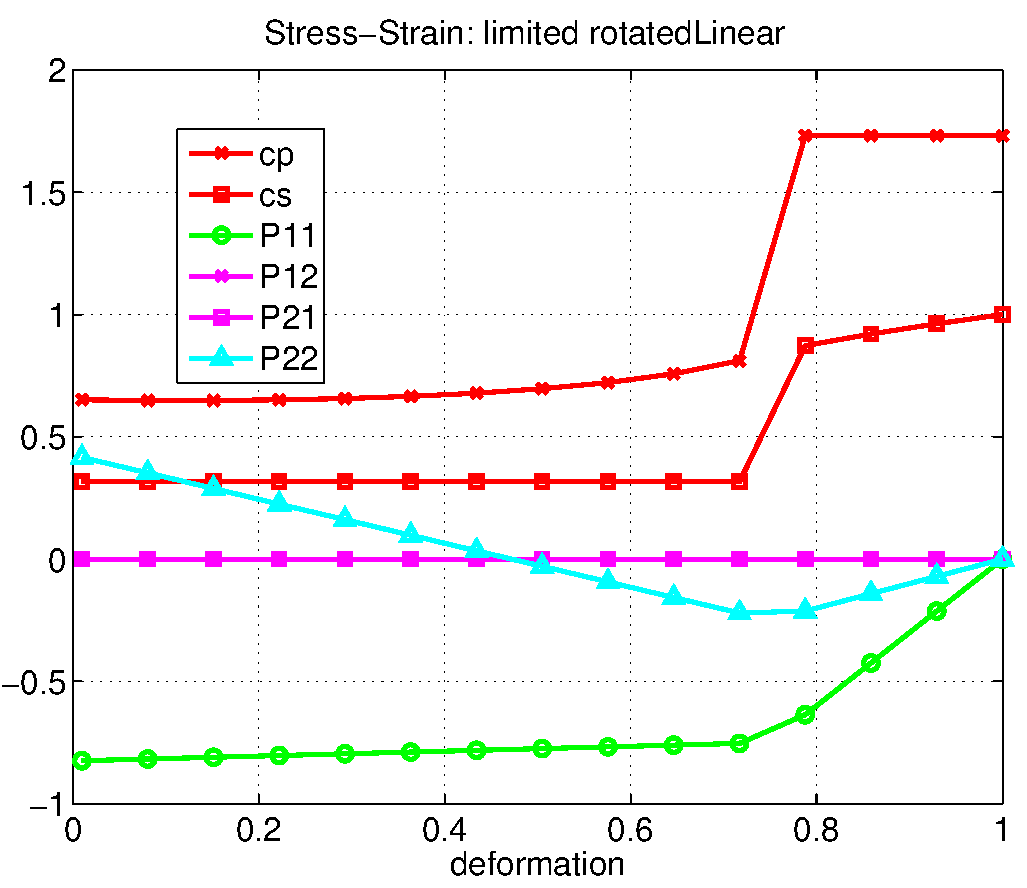
\includegraphics[width=\graphWidth]{fig/rotatedLinearlimitedStressStrain}
  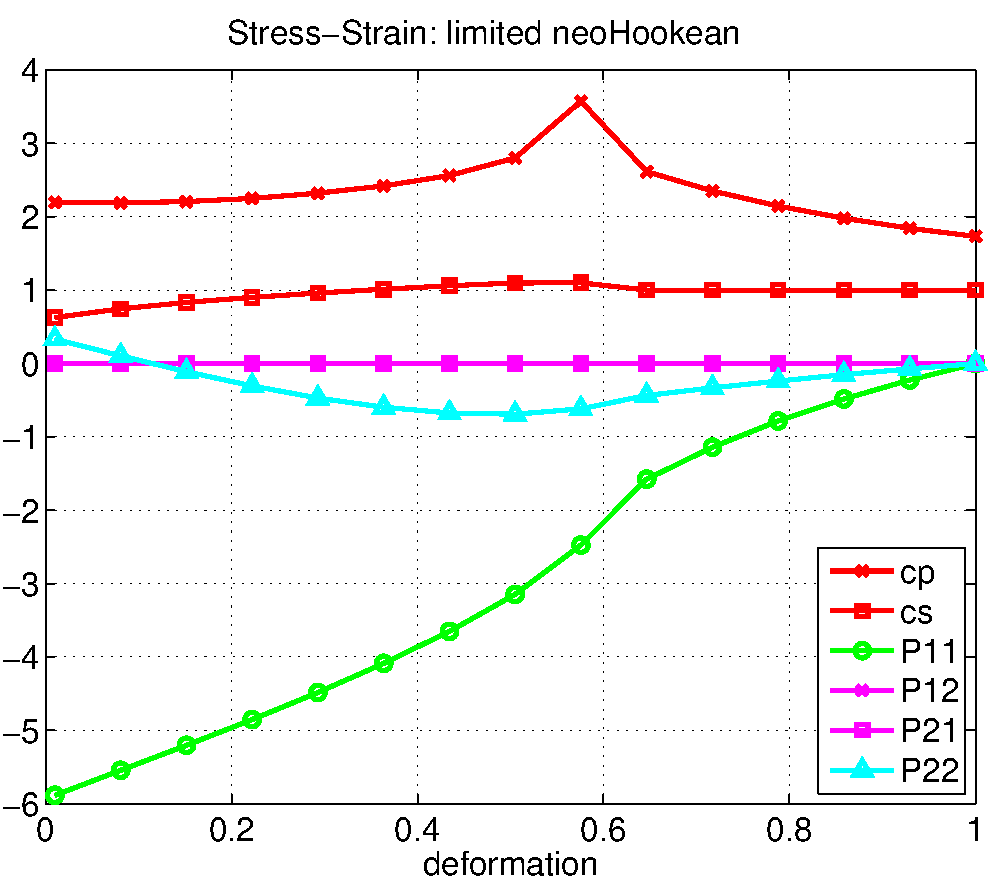
\includegraphics[width=\graphWidth]{fig/neoHookeanlimitedStressStrain}
  \caption{Limited stress-strain models.}
  \label{fig:largeStressStrainLimited}
\end{center}
\end{figure}
}


\paragraph{Some analysis.}
   For the case of a one-dimensional compression the wave speeds $c_p^2$ and $c_s^2$ are eigenvalues of the
matrix A: (where in the 1D case the off-diagonal terms will be zero)
\begin{align}
   A_{ij} = K_{1ij1} = \frac{\partial P_{1i}}{\partial F_{j1}}
\end{align}
% See cgDoc/sm/eigs.maple and eigs.out 
%  A[1,1]=((lam*F11+2*mu*F11)*F11+lam*(1/2*F11^2+1/2*F21^2-1+1/2*F12^2+1/2*F22^2)+2*mu*(1/2*F11^2+1/2*F21^2-1/2)+mu*F12^2)*k1^2
%  A[2,2]=((lam*F21+2*mu*F21)*F21+lam*(1/2*F11^2+1/2*F21^2-1+1/2*F12^2+1/2*F22^2)+2*mu*(1/2*F11^2+1/2*F21^2-1/2)+mu*F22^2)*k1
For the SVK model we have (*check me*)
\begin{align}
    c_p^2 &= A_{11} = \frac{\partial P_{11}}{\partial F_{11}} = (\lambda+2\mu) F_{11}^2  + \mu F_{12}^2 + S_{11}, \\
    c_s^2 &= A_{22} = \frac{\partial P_{12}}{\partial F_{21}} = (\lambda+2\mu) F_{21}^2  + \mu F_{22}^2 + S_{11}, \\
   S_{11} &= \half\lambda( F_{11}^2 + F_{12}^2+ F_{22}^2  + F_{21}^2 -2 ) + \mu( F_{11}^2 + F_{21}^2 -1 ), 
%          &= (\lambda+2\mu)( \half(F_{11}^2 + F_{21}^2 -1) ) + \lambda( \half(F_{22}^2+F_{12}^2))
\end{align}
Note that for $F_{11}\rightarrow 0$, $F_{22}=1$, $F_{12}=F_{21}=0$ (
i.e. large one-dimensional compression), $A_{11}$ and $A_{22}$ become negative since $S_{11}\sim -\lambda-\mu $ is negative.
In particular $A_{11}=0$ at $F_{11}=1/\sqrt{3}\approx .577$ and $A_{22}=0$ at $F_{11}=\sqrt{\lambda/(\lambda+2\mu)}$.
The scheme is no-longer hyperbolic when this occurs.

For the neo-Hooklean model we have (check me)
\begin{align}
   P_{11} &= \lambda \ln( J ) \frac{F_{22}}{J} + \mu( F_{11} - \frac{F_{22}}{J}, \\
   P_{12} &= \lambda \ln( J ) \frac{(-F_{21})}{J} + \mu( F_{21} + \frac{F_{12}}{J}), \\
   J &= F_{11}F_{22} -F_{12} F_{21} .
\end{align}
whence, (*check me*)
\begin{align}
 c_p^2  = \frac{\partial P_{11}}{\partial F_{11}} &= \lambda\Big( (1-\ln(J)) \frac{F_{22}^2}{J^2}\Big) + \mu( 1 + \frac{F_{22}^2}{J^2} ), \\
 c_s^2 = \frac{\partial P_{12}}{\partial F_{21}} &= \lambda\Big( (1-\ln(J))\frac{F_{12} F_{21}}{J^2} - \ln(J)\frac{1}{J} \Big)
         + \mu( 1 + \frac{F_{12}^2}{J} )
\end{align}
We see that for a material under compression, $0<J<1$, $\ln(J)<0$ and both $c_p^2$ and $c_s^2$ remain positive. 

For the {\bf rotated-linear} model, {\bf **Finish me**}
\begin{align}
  \Fv &= \Uv \Fvhat \Vv^T \quad{(SVD)} ,  \\
  \Pvhat &= \lambda tr(\Fvhat-\Iv)\Iv + 2\mu( \Fvhat -\Iv), \\ 
         &= \diag(\Phat_1,\Phat_2), \\
  \Pv &= \Uv \Pvhat \Vv^T \\
  P_{ij} &= U_{im} \Phat_m V_{jm}
\end{align}
where $\Fvhat=\diag(\sigma_1,\sigma_2)$ with
\begin{align}
   \sigma_1^2 &= \sigma_1^2(\Fv)
\end{align}
and
\begin{align}
   \frac{\partial P_{ij}}{\partial F_{kl}} &= 
\end{align}
